\documentclass[a4paper,11pt]{report}
\usepackage{chuan_math_gkt}
\usetikzlibrary{angles,quotes,intersections,patterns,decorations.pathreplacing}
\chuanexamsetup

\begin{document}
\examfontsize

\examsecret{绝密$\bigstar$启用前}

\examtitle{2021年普通高等学校招生全国统一考试（新高考I卷）}{数\quad 学}

\noticetitle
\begin{examnotice}
\item 答卷前，考生务必将自己的姓名、准考证号填写在答题卡上。
\item 回答选择题时，选出每小题的答案后，用铅笔把答题卡上对应题目的答案标号涂黑。如需改动，用橡皮擦干净后，再选涂其他答案标号。回答非选择题时，将答案写在答题卡上。写在本试卷上无效。
\item 考试结束后，将本试卷和答题卡一并交回。
\end{examnotice}
\examsection{一、选择题：本题共8小题，每小题5分，共40分。在每小题给出的四个选项中，只有一项是符合题目要求的。}
\begin{examquestions}

\item 
设集合$A=\{x|-2<x<4|\}$，$B=\{2,3,4,5\}$，则$A\cap B=$

\fourchoices{$\{2\}$}{$\{2,3\}$}{$\{3,4\}$}{$\{2,3,4\}$}

\item 
已知$z=2-i$，则$z(\overline{z}+i)=$

\fourchoices{$6-2i$}{$4-2i$}{$6+2i$}{$4+2i$}

\item 
已知圆锥的底面半径为$\sqrt{2}$，其侧面展开图为一个半圆，则该圆锥的母线长为

\fourchoices{$2$}{$2\sqrt{2}$}{$4$}{$4\sqrt{2}$}

\item 
下列区间中，函数$f(x)=7sin(x-\dfrac{\pi}{6})$单调递增的区间是

\onechoices{$(0,\dfrac{\pi}{2})$}{$(\dfrac{\pi}{2},\pi)$}{$(\pi,\dfrac{3\pi}{2})$}{$(\dfrac{3\pi}{2},2\pi)$}

\item 
已知$F_{1}$，$F_{2}$是椭圆$C$：$\dfrac{x^{2}}{9}+\dfrac{y^{2}}{4}=1$的两个焦点，点$M$在$C$上，则$|MF_{1}|\cdot|MF_{2}|$的最大值为

\fourchoices{13}{12}{9}{6}

\item 
若$\tan\theta=-2$，则$\dfrac{\sin\theta(1+sin2\theta)}{\sin\theta+\cos\theta}=$

A
$-\dfrac{6}{5}$
B.
$-\dfrac{2}{5}$
C.
$\dfrac{2}{5}$
D.
$\dfrac{6}{5}$

\item 
若过点$(a,b)$可以作曲线$y=e^{x}$的两条切线，则

\fourchoices{$e^{b}<a$}{$e^{a}<b$}{$0<a<e^{b}$}{$0<b<e^{a}$}

\item 
有6个相同的球，分别标有数字1，2，3，4，5，6，从中有放回的随机取两次，每次取1个球，甲表示事件``第一次取出的球的数字是1''，乙表示事件``第二次取出的球的数字是2''，丙表示事件``两次取出的球的数字之和是8''，丁表示事件``两次取出的球的数字之和是7''，则

\fourchoices{甲与丙相互独立}{甲与丁相互独立}{乙与丙相互独立}{丙与丁相互独立}

\item 
有一组样本数据$x_{1}$，$x_{2}$，\ensuremath{\ldots}，$x_{n}$，由这组数据得到新样本数据$y_{1}$，$y_{2}$，\ensuremath{\ldots}，$y_{n}$，其中$y_{i}=x_{i}+c$($i=1,2,\cdot\cdot\cdot,n),c$为非零常数，则

\graphchoices
{两组样本数据的样本平均数相同}
{两组样本数据样本中位数相同}
{两组样本数据的样本标准差相同}
{两组样数据的样本极差相同}

\item 
已知$O$为坐标原点，点$P_{1}(\cos\alpha,\sin\alpha)$，$P_{2}(\cos\beta,-\sin\beta)$，$P_{3}(\cos(\alpha+\beta),\sin(\alpha+\beta))$，$A(1,0)$，则

\fourchoices{$|\vec{OP_{1}}|=|\vec{OP_{2}}|$}{$|\vec{AP_{1}}|=|\vec{AP_{2}}|$}{$\vec{OA}\cdot\vec{OP}_{3}=\vec{OP_{1}}\cdot\vec{OP_{2}}$}{$\vec{OA}\cdot\vec{OP_{1}}=\vec{OP_{2}}\cdot\vec{OP_{3}}$}

\item 
已知点$P$在圆$(x-5)^{2}+(y-5)^{2}=16$上，点$A(4,0)$、$B(0,2)$，则

\fourchoices{点$P$到直线$AB$的距离小于$10$}{点$P$到直线$AB$的距离大于$2$}{当$\angle PBA$最小时，$|PB|=3\sqrt{2}$}{当$\angle PBA$最大时，$|PB|=3\sqrt{2}$}

\item 
在正三棱柱$ABC-A_{1}B_{1}C_{1}$中，$AB=AA_{1}=1$，点$P$满足$\vec{BP}=\lambda\vec{BC}+\mu\vec{BB_{1}}$，其中$\lambda\ensuremath{\in}[0,1]$，$\mu\ensuremath{\in}[0,1]$，则

\onechoices{当$\lambda=1$时，$\ensuremath{\triangle}AB_{1}P$的周长为定值}{当$\mu=1$时，三棱锥$P-A_{1}BC$的体积为定值}{当$\lambda=\dfrac{1}{2}$时，有且仅有一个点$P$，使得$A_{1}P\ensuremath{\perp} BP$}{当$\mu=\dfrac{1}{2}$时，有且仅有一个点$P$，使得$A_{1}B\ensuremath{\perp}$平面$AB_{1}P$}

\item 
已知函数$f(x)=x^{3}(a\cdot2^{x}-2^{-x})$是偶函数，则$a=$\_\_\_\_\_\_.

\item 
已知$O$为坐标原点，抛物线$C$：$y^{2}=2px$($p>0$)的焦点为$F$，$P$为$C$上一点，$PF$与$x$轴垂直，$Q$为$x$轴上一点，且$PQ\ensuremath{\perp} OP$，若$|FQ|=6$，则$C$的准线方程为\_\_\_\_\_\_.

\item 
函数$f(x)=|2x-1|-2\ensuremath{\ln x}$的最小值为\_\_\_\_\_\_.

\item 
某校学生在研究民间剪纸艺术时，发现剪纸时经常会沿纸的某条对称轴把纸对折，规格为$20dm\times12dm$的长方形纸，对折1次共可以得到$10dm\times12dm$，$20dm\times6dm$两种规格的图形，它们的面积之和$S_{1}=240dm^{2}$，对折2次共可以得到$5dm\times12dm$，$10dm\times6dm$，$20dm\times3dm$三种规格的图形，它们的面积之和$S_{2}=180dm^{2}$，以此类推，则对折4次共可以得到不同规格图形的种数为\_\_\_\_\_\_；如果对折$n$次，那么$S_{k}k=1n\sum=$\_\_\_\_\_\_$dm^{2}$.

\end{examquestions}
\examsection{四、解答题：本题共6小题，共70分。解答应写出文字说明、证明过程或演算步骤。}
\begin{examanswers}[start=17]

\item（10分）

已知数列$\{a_{n}\}$满足$a_{1}=1$，$a_{n+1}=\{\begin{matrix}a_{n}+1,n为奇数,\\\end{matrix}a_{n}+2,n为偶数.\}\{$

（1）记$b_{n}=a_{2n}$，写出$b_{1}$，$b_{2}$，并求数列$\{b_{n}\}$的通项公式；

（2）求$\{a_{n}\}$的前20项和.

\item（12分）

某学校组织``一带一路''知识竞赛，有\emph{A}，\emph{B}两类问题，每位参加比赛的同学先在两类问题中选择一类并从中随机抽取一个问题回答，若回答错误则该同学比赛结束：若回答正确则从另一类问题中再随机抽取一个问题回答，无论回答正确与否，该同学比赛结束.\emph{A}类问题中的每个问题回答正确得20分，否则得0分：\emph{B}类问题中的每个问题回答正确得80分，否则得0分，己知小明能正确回答\emph{A}类问题的概率为0.8，能正确回答\emph{B}类问题的概率为0.6，且能正确回答问题的概率与回答次序无关.

（1）若小明先回答\emph{A}类问题，记$X$为小明的累计得分，求$X$的分布列；

（2）为使累计得分期望最大，小明应选择先回答哪类问题？并说明理由.

\item（12分）

记$\ensuremath{\triangle}ABC$是内角$A$，$B$，$C$的对边分别为$a$，$b$，$c$.已知$b^{2}=ac$，点$D$在边$AC$上，$BD\sin\angle ABC=a\ensuremath{\sin C}$.

（1）证明：$BD=b$；

（2）若$AD=2DC$，求$\cos\angle ABC$.

\item（12分）

如图，在三棱锥$A-BCD$中，平面$ABD\ensuremath{\perp}$平面$BCD$，$AB=AD$，$O$为$BD$的中点.

\noindent\begin{minipage}[t]{0.62\linewidth}
（1）证明：$OA\ensuremath{\perp} CD$；

（2）若$\ensuremath{\triangle}OCD$是边长为1等边三角形，点$E$在棱$AD$上，$DE=2EA$，且二面角$E-BC-D$的大小为$45^\circ$，求三棱锥$A-BCD$的体积.
\end{minipage}\hfill
\begin{minipage}[t]{0.32\linewidth}\vspace{-1.2em}\centering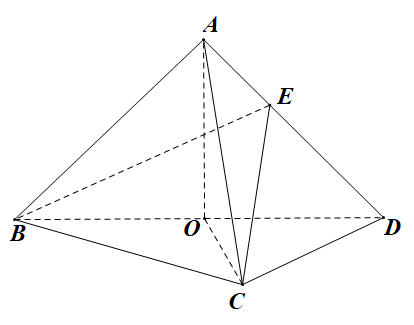
\includegraphics[width=\linewidth]{figures/2021_xgk1_image131.png}\end{minipage}
\item（12分）

在平面直角坐标系$xOy$中，已知点$F_{1}(-\sqrt{17},0)$、$F_{2}(\sqrt{17},0)|MF_{1}|-|MF_{2}|=2$，点$M$的轨迹为$C$.

（1）求$C$的方程；

（2）设点$T$在直线$x=\dfrac{1}{2}$上，过$T$两条直线分别交$C$于$A$、$B$两点和$P$，$Q$两点，且$|TA|\cdot|TB|=|TP|\cdot|TQ|$，求直线$AB$的斜率与直线$PQ$的斜率之和.

\item（12分）

已知函数$f(x)=x(1-\ensuremath{\ln x})$.

（1）讨论$f(x)$的单调性；

（2）设$a$，$b$为两个不相等的正数，且$b\ensuremath{\ln a}-a\ensuremath{\ln b}=a-b$，证明：$2<\dfrac{1}{a}+\dfrac{1}{b}<e$.
\end{examanswers}

\end{document}
